\section{Continuous Training Approach} \label{continuous-training-serving}
\todo[inline]{This chapter is completely new. So I won't highlight it.}
\begin{figure*}[t]
\centering
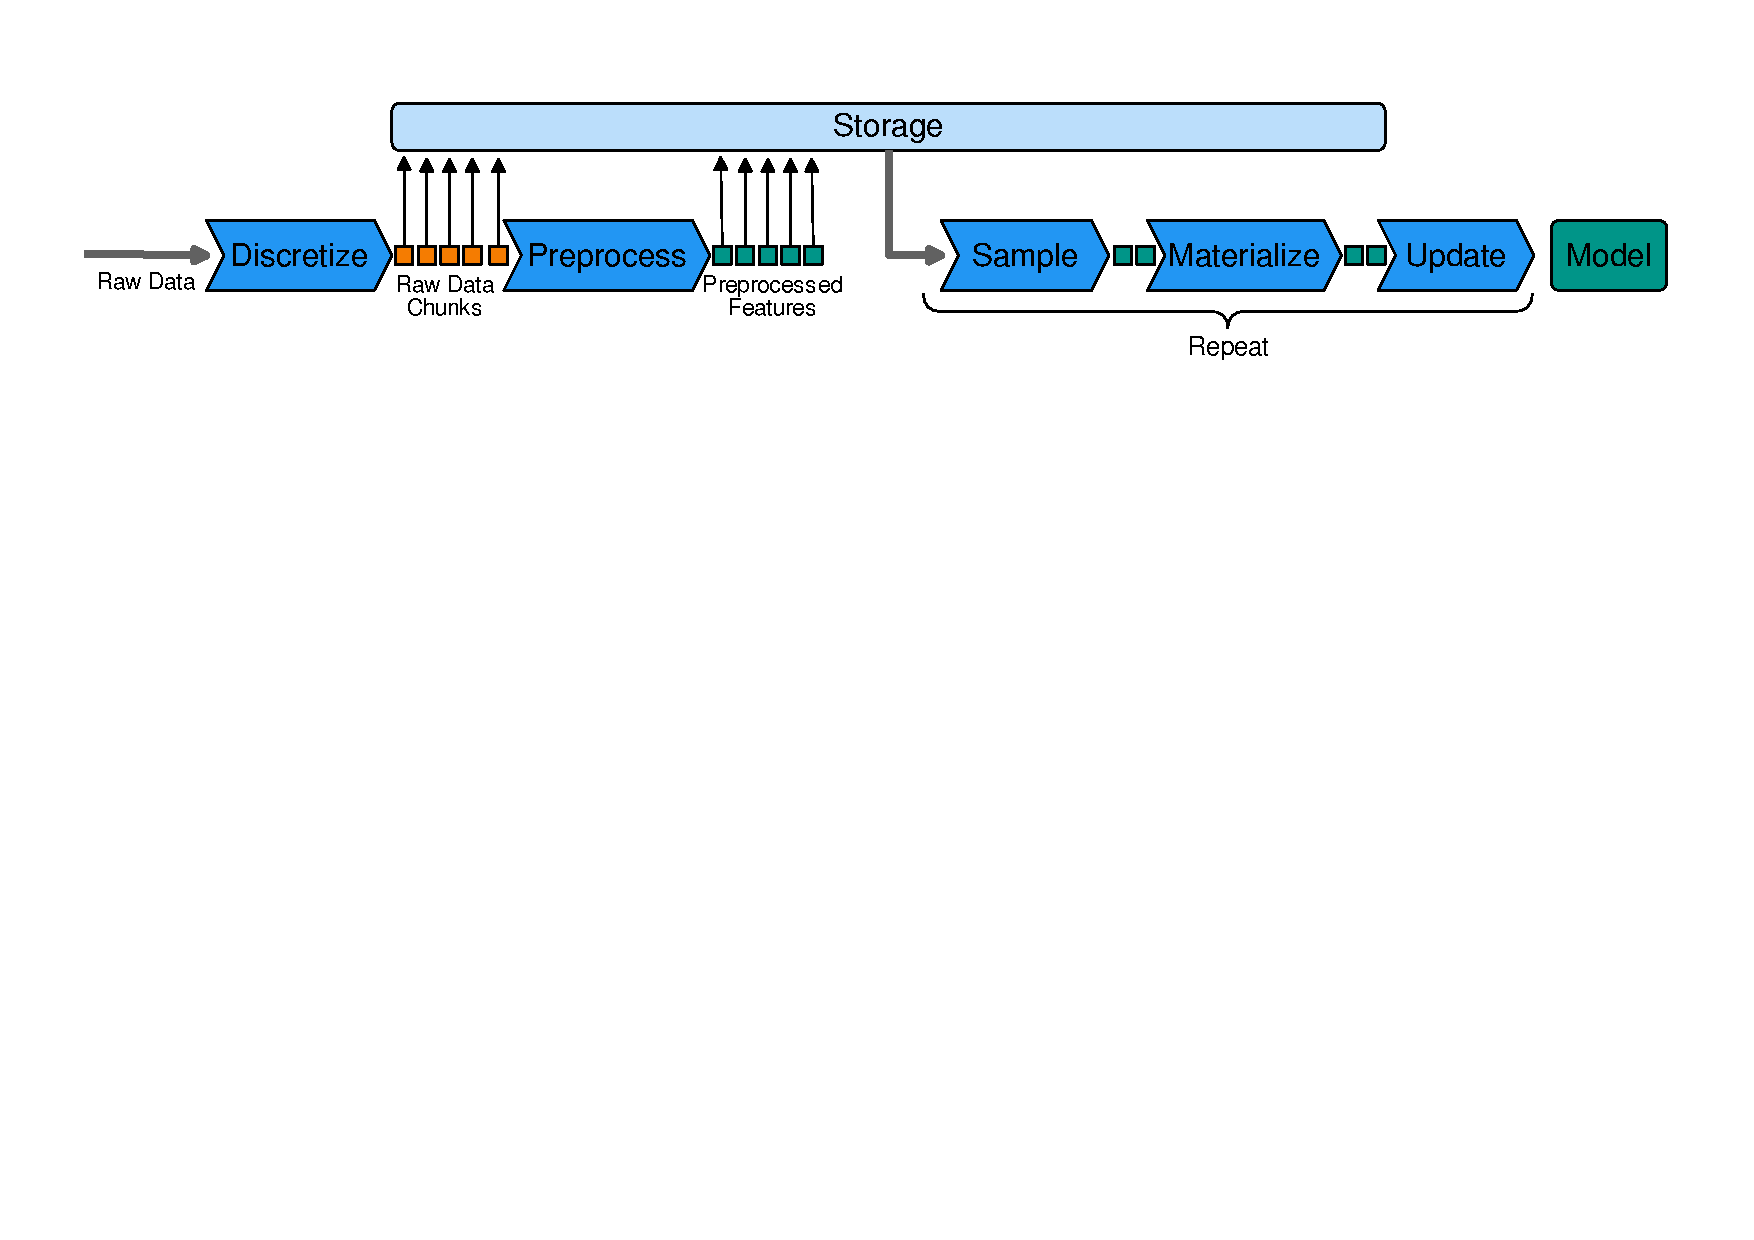
\includegraphics[width=\textwidth]{../images/continuous-training-details.pdf}
\caption{Workflow of our continuous deployment approach. (1) The platform converts the data into small units (2) The platform utilizes the deployed pipeline to preprocess the data and transform the raw data into features and store them in the storage. (3) The platform samples the data from the storage. (4) The platform materializes the sampled data (5) Using the sampled data, the deployment platform updates the deployed model.}
\label{fig:continuous-deployment-details}
\end{figure*}

In this section, we describe the details of our continuous training approach.
Figure \ref{fig:continuous-deployment-details} shows the workflow of our proposed platform.
The platform processes the incoming training data through 5 stages:\newline
\textbf{1. Discretizing the data: } 
To efficiently preprocess the data and update the model, the platform transforms the data into small chunks and stores them in the storage unit. 
The platform assigns a timestamp to every chunk indicating their creation time.
The timestamp acts as both a unique identifier and an indicator of the recency of the chunk.\newline
\textbf{2. Preprocessing the data: } 
The platform utilizes the deployed pipeline to preprocess the raw training data chunks and transform them into feature chunks.
Then, the platform stores the feature chunks along with a reference to the originating raw data chunk in the storage unit.
During the preprocessing stage, we utilize \textit{online statistics computation} to compute the required statistics for the different pipeline components.
These statistics speed up the data processing in later stages.
When the storage unit becomes full, the platform starts removing the oldest feature chunks and only keep the reference to the originating raw data chunks.
In case the later stages of the deployment platform request a deleted feature chunk, the platform can recreate the feature chunk by utilizing the referenced raw data chunk. \newline
\textbf{3. Sampling the data: }
A sampler unit samples the feature chunks from the storage.
Different sampling strategies are available to address different use-case requirements.\newline
\textbf{4. Materializing the data: }
Depending on the size of the storage unit, some preprocessed feature chunks (results of step 2) are not materialized.
If the sampler selects unmaterialized feature chunks, the platform recreates these feature chunks by utilizing the deployed pipeline through a process called \textit{dynamic materialization}.\newline
\textbf{5. Updating the model: }
By utilizing the preprocessed feature chunks, the platform updates the deployed model through a process called \textit{proactive training}.\newline

After the user designs and deploys the pipeline, we rely on the existing big data processing frameworks to perform the discretization and preprocessing.
The sampling strategy typically depends on the use-case.
However, different sampling strategies have different implications for the dynamic materialization process.
In the rest of this section, we first describe the details of the online statistics computation.
Then we introduce the dynamic materialization approach and the effects of different sampling strategies on the materialization process.
Finally, we describe the details of the proactive training method.

\subsection{Online Statistics Computation}\label{online-statistics-computation}
Some components of the machine learning pipeline, such as the standard scaler or the one-hot encoder, require some statistics of the dataset before they process the data.
Computing these statistics requires scans of the data.
In our deployment platform, we utilize online training as well as proactive training.
During the online update of the deployed model, we compute all the necessary statistics for every component.
Every pipeline component first reads the incoming data.
Then it updates its underlying statistics.
Finally, the component transforms and forwards the data to the next component.
Online computation of the required statistics eliminates the need to recompute the same statistics during the dynamic materialization and proactive training.

Online statistics computation is only possible for certain types of pipeline components.
The support for stateless pipeline operations is trivial.
These operations require no update.
They are only utilized to transform the data for the following pipeline components.
For stateful operations, since the statistics update occurs during the online data processing, the platform can only update the statistics that can be computed incrementally.
Many of the well-known data preprocessing components (such as standardization and one-hot encoding) require statistics that can be computed incrementally.
However, some pipeline components require statistics that cannot be updated incrementally (such as percentile).
For these types of statistics, the pipeline component has to rescan the entire data points whenever new data becomes available.
For such components, when possible, we can utilize probabilistic and approximate data structures (such as bloom filters or count-min sketch \cite{cormode2005improved}).
Otherwise, we do not provide support for deployment of pipelines containing components that require a scan of the entire historical data whenever new data becomes available.

The platform can also facilitate the online statistics computation for custom pipeline components.
In Section \ref{sec:system-architecture}, we describe how users can incorporate this feature into their custom pipeline components.

\subsection{Dynamic Materialization}\label{subsec:dynamic-materialization}
In order to update the statistics of the pipeline components, each component must transform the data and passes it to the next component.
At the end of this process, the pipeline has transformed the data chunks into feature chunks that the model will utilize during the training process.
In our continuous training platform, we repeatedly sample the feature chunks to update the model.
Storing the chunks as materialized features greatly reduces the processing time as the entire data preprocessing steps can be skipped during the model update.
However, in presence of a limited storage capacity, one has to consider the effect of storing the materialized feature chunks.

To address the storage capacity issue, we utilize dynamic materialization.
While creating the feature chunks, the platform assigns a unique identifier (the creation timestamp) and a reference to the raw data chunk.
In dynamic materialization, when the size of the store feature chunks exceeds the storage capacity, the platform removes the content of the oldest materialized feature chunks from the storage and only keeps the unique identifier and the reference to the raw data chunk (similar to cache eviction).
The next time the sampler selects one or more of the evicted feature chunks, the platform re-materializes each feature chunk from the raw data chunk by utilizing the deployed pipeline.
Figure \ref{fig:dynamic-materialization-process} shows the process of dynamic materialization in two possible scenarios.
For both scenarios, there are a total 6 data chunks (raw and feature) available in the storage (with timestamps $t_0$ to $t_5$).
The sampling operation selects the chunks at $t_0$, $t_2$, and $t_5$.
In the first scenario (left), the feature chunks are all materialized.
Therefore, the platform directly utilizes them to update the model.
In the second scenario (right), the platform has previously evicted some of the materialized feature chunks due to the limit on the storage capacity.
In this scenario, the platform first re-materializes the evicted chunks using the deployed pipeline components before updating the model.

\begin{figure}[h]
\centering
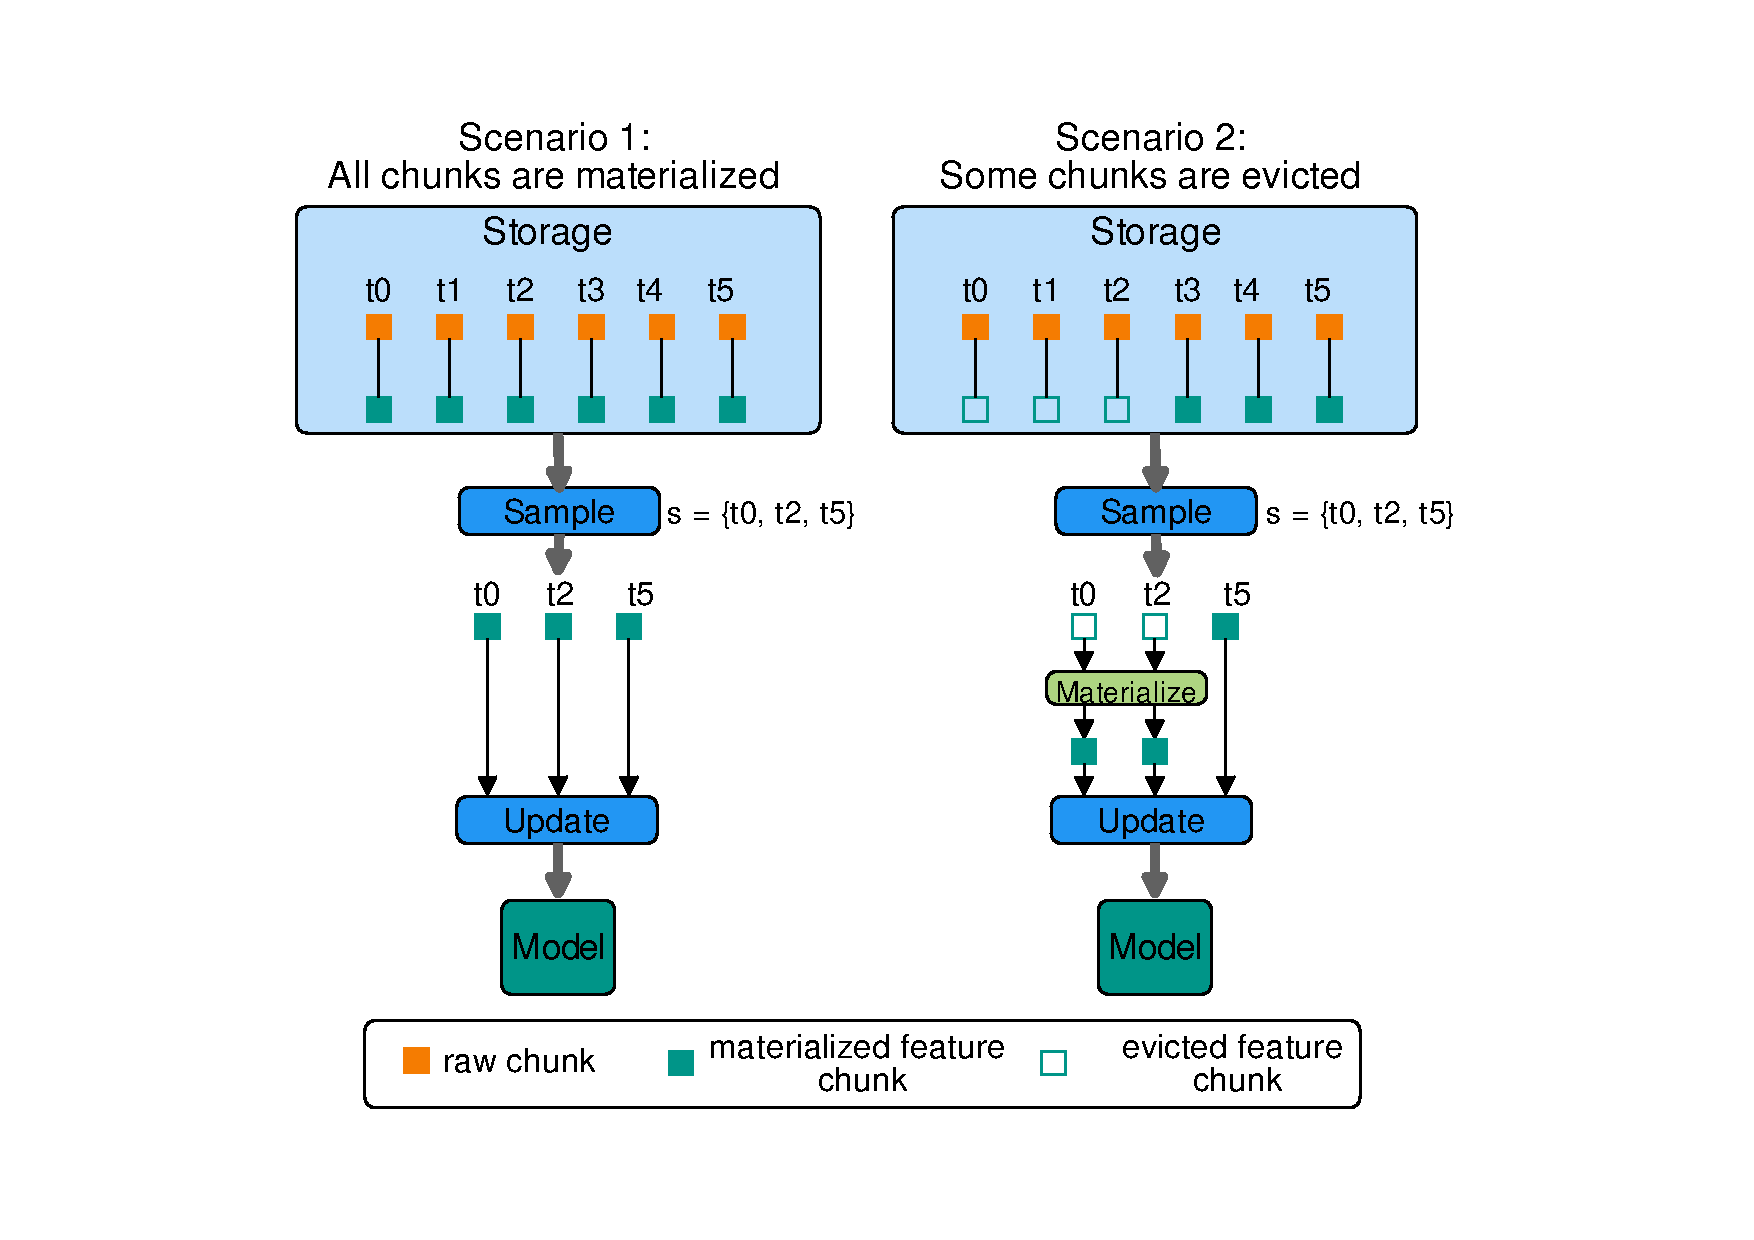
\includegraphics[width=\columnwidth]{../images/dynamic-materialization.pdf}
\caption{Dynamic Materialization process. (left) all feature chunks are materialized. (right) some feature chunks are evicted}
\label{fig:dynamic-materialization-process}
\end{figure}
It is important to note that the continuous training platform assumes the raw data chunks are always stored and are available for re-materialization.
If some of the raw data chunks are not available, the platform ignores these chunks during the sampling operation.
A similar issue arises in the periodical deployment approach.
If there is not enough space to store all the historical and incoming data, at every retraining, the platform only utilizes the available data in the storage.

\subsubsection{Storage requirement for materialized feature chunks.} 
In order to estimate the storage requirement for the preprocessed feature chunks, we investigate the storage complexity of different pipeline components in terms of the input size (raw data chunks).
Table \ref{pipeline-component-description} shows the categories of the pipeline components and their characteristics.
\begin{table}[h!]
\centering
\begin{tabular}{lll}
\hline
\textbf{Component type}  & \textbf{Unit of work} &\textbf{Characteristics}  \\
\hline
data transformation			& data point (row)       	  & filtering or        \\
			&  	  &  one-to-one mapping        \\
feature selection            & feature (column)             & selecting a subset of   \\
			&  	  &   the columns        \\
feature extraction & feature (column) & creating new columns \\
\hline
\end{tabular}
\caption{Description of the pipeline component types. Unit of work: \textit{row} indicates the component operates on one or multiple rows at a time, \textit{column} indicates the component operates on one or multiple columns at a time}  
\label{pipeline-component-description}
\end{table}
Assuming the size of the input data is $n$, the storage complexity of data transformation and feature selection operations are linear in terms of the input size ($O(n)$).
This is because these operations either perform a one-to-one mapping (normalization) or reduce the size of the data (anomaly filtering and feature selection).
The case for feature extraction is more complicated as there are different types of feature extraction operations.
In many cases, the feature extraction process creates a new feature by combining one or more existing features (such as summing or multiplying features together).
In these cases, the storage complexity is $O(n)$ as the increase in size is linear with respect to the input size.
In some cases, the feature extraction process may generate many features from a small subset of the existing features.
Prominent examples of such operations are one-hot encoding and feature hashing.
One-hot encoding converts a column of the data with categorical values into several columns (1 column for each unique value).
For every value in the original column, the encoded representation has the value of $1$ in the column the value represents and $0$ in all the other columns.
Let us assume the number of the unique values in the column is $m$.
Thus, the storage complexity of the one-hot encoding operation is $O(mn)$.
Based on the value of $m$, three scenarios can occur:
\begin{itemize}
\item if $m \ll n$, then the storage complexity is $O(n)$
\item if $m \approx n$, then the storage complexity is $O(n^2)$
\item if $m \gg n$, then the storage complexity is $\Omega (n^2)$
\end{itemize}
In the first two cases, we have an upper bound on the storage requirements.
However, the last case is data-dependent and the size of the materialized features may have a polynomial growth rate with respect to the size of the original data, which may render storage of even a few features chunks impossible.
However, both one-hot encoding and feature hashing produce sparse data.
Therefore, by utilizing sparse data representation, we can guarantee a storage complexity of $O(n)$ in all three cases.

Since the storage requirement is in worst-case scenario linear with respect to the size of the raw data and the eviction policy gradually dematerializes the older feature chunks, we can safely assume the size of the materialized features will not exceed the storage capacity.

\subsubsection{Effects of sampling strategies on the dynamic materialization.}
The choice of the sampling strategy affects the efficiency of the dynamic materialization.
Here, we analyze the effects of dynamic materialization in reducing the data processing overhead.

We define $n$ as the total number of the feature chunks, $m$ as the number of the materialized feature chunks, and $s$ as the number of the sample size, where $s < m < n$. 
To quantify the efficiency of the dynamic materialization, we introduce the materialization utilization rate:
\begin{center}
 $MU = \dfrac{E[mc]}{s}$
\end{center}
where $mc$ is the number of the materialized chunks.
The materialization utilization rate indicates the ratio of the feature chunks that do not require re-materialization before updating the model (a $MU$ of $0.5$ indicates that on average half of the sampled chunks do not need to be re-materialized before updating the model).

The variable $mc$ follows a hypergeometric distribution\footnote{https://en.wikipedia.org/wiki/Hypergeometric\_distribution} (sampling without replacement) where the number of success states is $m$, the population size is $n$, and the number of draws is $s$.
The expected value of the hypergeometric is:
\begin{center}
$E[mc] = s\dfrac{m}{n}$
\end{center}
Therefore, the materialization utilization rate can be computed as: 
\begin{equation} \label{formula-mu}
MU = \dfrac{s\dfrac{m}{n}}{s} = \frac{m}{n}
\end{equation}

\textbf{Random Sampling:} 
For the random sampling strategy, we can directly use Formula \ref{formula-mu} to compute the materialization utilization rate.

\textbf{Window-based Sampling:}
In window based sampling, we have an extra parameter $w$ which indicates the number of chunks in the active window.
Therefore, in Formula \ref{formula-mu}, we have to replace the population size $n$ with the window size $w$.
Therefore, the materialization utilization rate is: 
\begin{equation}
MU = \dfrac{m}{w}
\end{equation}

\textbf{Time-based Sampling:}
In time-based sampling, we assign a weight to each chunk indicating how recent the data has arrived at the system.
Therefore, for the $n$ chunks, the weights are assigned using the following formula:
\begin{equation} \label{formula-weight}
w_i = \dfrac{i}{\dfrac{n(n+1)}{2}}, \ i = 1 ... n
\end{equation}
which ensures the sum of the all the weights is equal to 1.
To compute the materialization utilization ratio, we have to $m$ with the sum of the weights of the materialized items ($\sum_{i=n-m+1}^{n} w_i$) and replace $n$ with the sum of all the weights ($\sum_{i=1}^{n} w_i\ = 1$).
\begin{equation}
\begin{aligned}
MU &= \dfrac{\sum_{i=n-m+1}^{n} w_i}{1}\\
&=\dfrac{n-m+1}{\dfrac{n(n+1)}{2}} + ... + \dfrac{n}{\dfrac{n(n+1)}{2}} \\
&= \dfrac{m(2n-m+1)}{n(n+1)}
\end{aligned}
\end{equation}

\textbf{An example use-case:}
To demonstrate with a real use-case, consider a storage system of a total of 120 GB.
We divide the data into chunks of 1 MB. 
Let's assume $n=10000$ (100 GB), $m=2000$ (20 GB), $w=5000$, and $s=100$.
With these values, the materialization utilization $MU$ is $0.2$, $0.4$, and $0.345$ for the random, window-based, and time-based sampling respectively.
The theoretical analysis in this section provides an estimate of how much the dynamic optimization can reduce the processing overhead.
In our experiments, we also empirically show the effect of dynamic optimization on real-world datasets.

\subsection{Proactive Training}\label{proactive-training}
Updating the model is the last step of our continuous deployment platform.
We update the model through the proactive training process.
Unlike, the full retraining process that is triggered by a certain event (such as a drop in the quality or certain amount of time elapsed since the last retraining), proactive training continuously updates the deployed model.
The proactive training utilizes the mini-batch stochastic gradient descent to update the model incrementally.
Each instance of the proactive training is analogous to an iteration of the mini-batch SGD.
Algorithm \ref{mini-batch-SGD} shows the pseudocode of the mini-batch SGD algorithm.
\begin{algorithm}
\caption{mini-batch Stochastic Gradient Descent}\label{mini-batch-SGD}
\begin{algorithmic}[1]
\Require  $D=$ training dataset
\Ensure $m=$ trained model
\For {$i = 1 ... N$}
	\State $s_i =$ sample from $D$
	\State $g = \nabla J(s_i, \textcolor{blue}{m_{i-1}})$
	\State $m_i = \textcolor{blue}{m_{i-1}} - \textcolor{blue}{\eta_{i-1}}g$
\EndFor
\end{algorithmic}
\end{algorithm}

Since the platform executes the proactive training in arbitrary intervals, we must ensure each instance of the proactive training is independent of the previous instances.
According to the mini-batch SGD algorithm, each iteration of the SGD only requires the model parameters ($m_{i-1}$) and the learning rate parameters ($\eta_{i-1}$) of the previous iterations (line 3 and 4).
Given these parameters, iterations of SGD are conditionally independent of each other.
In order to execute the proactive training, the deployment platform only needs to store the model parameters (model weight vector) and the learning rate parameters (past gradients and momentum vectors for the advanced learning rate adaptation methods).
By proactively training the deployed model, the platform ensures the model stays up-to-date and provides accurate predictions.

Proactive training is a form of incremental training \cite{gepperth2016incremental} which is limited to SGD-based models.
In our deployment platform, one can replace the proactive training with other forms of incremental training.
However, we limit the platform's support to SGD for two reasons.
First, SGD is simple to implement and is used for training a verity of machine learning models in different domains \cite{ macmahan2013, bottou1995convergence, koren2009matrix,  funk2006netflix}. 
Second, since the combination of the data sampling and the proactive training is similar to the mini-batch SGD procedure, proactive training provides the same regret bound on the convergence rate as the existing stochastic optimization approaches \cite{zhang2004solving, kingma2014adam}.

%\subsection{Proactive Training} \label{proactive-training}
%Proactive training is a replacement for the periodical retraining of the deployed model.
%Typically, the retraining is triggered when a condition is met, e.g., the quality of the model drops below a certain value.
%Contrary to the periodical training, in proactive training, the platform continuously update the deployed model using the historical data.
%
%We take advantage of the iterative nature of SGD in the design of the proactive training.
%The input to each iteration of SGD is the current weight parameters of the model, a sample of the data points, and an objective function.
%In proactive training, we execute iterations of mini-batch SGD on the deployed model.
%To execute the proactive training, the deployment platform first samples the historical data.
%Then, the platform transforms the data into a set of features using the deployed pipeline.
%Next, the proactive trainer utilizes the transformed features to compute the gradient of the objective function.
%Finally, the deployment platform updates the deployed model using the computed gradient.
%
%The learning rate parameter of SGD has a significant impact on the proactive training.
%To effectively update the deployed model, one has to tune the learning rate.
%Similar to the offline SGD, using a constant or decreasing value for the learning rate results in suboptimal training.
%Adaptive learning rate methods work well in a dynamic environment where the distribution of the data may change over time \cite{zeiler2012adadelta}.
%Therefore, in proactive training, instead of using simple learning rate tuning mechanisms, we utilize the more advanced learning rate adaptation methods.
%The performance of the different learning rate adaptation techniques varies across different datasets.
%To choose the most promising adaptation technique, we rely on hyperparameter tuning during the initial model training on the historical dataset \cite{bergstra2012random}.
%After the initial training, the deployment platform selects the same learning rate adaptation technique for the proactive training.
%Our experiments in Section \ref{evaluation} show that selecting the adaptation technique based on initial training results in a model with the highest quality during the proactive training.
%
%The proactive training aims to adapt the deployed model to the recent data items.
%As a result, when sampling the historical data, one has to consider the effect of the sample on the deployed model.
%In Section \ref{sec:system-architecture}, we explain the different sampling strategies.
%A time-based sampling approach of the historical data emphasizes the more recent data points and adapts the deployed model to the changes in the data distribution.
%In Section \ref{evaluation}, we evaluate the quality of the deployed model when different sampling techniques are utilized (time-based, uniform, and window-based).
%We show that the time-based sampling results in a model with better quality.
%\textit{Model Stability}
%To ensure that proactive training does not degrade the quality of the model, a model evaluator is used to assess the quality of the model.
%The proactive trainer uses the latest deployed model as an initial starting point and updates the model based on the training data.
%The evaluator assesses the quality of the model using an evaluation dataset or the prequential evaluation method \cite{dawid1984present}.
%If the quality of the model has degraded, the update is discard and the model is logged.
%This is to avoid over training the deployed model in proactive training.
%\todo[inline]{I'm going to remove scheduling rate and just run proactive training when the sample buffer is full}
%\textit{Scheduling rate.}
%\hl{An extra parameter of proactive training is the scheduling rate.
%In offline training, iterations of SGD are executed one after the other until convergence.
%In proactive training, the scheduling rate defines the frequency of SGD iteration execution.
%The scheduling rate plays an important role as it directly affects the freshness of the deployed model.
%However, a high scheduling rate results in many frequent SGD iterations which incur an overhead on the deployment system as it is using a lot of resources.
%A small scheduling rate also affects the model freshness.
%To increase the efficiency of the system a scheduler component is designed that is tasked with scheduling new iterations of SGD.
%Similar to learning rate tuning, we use an adaptive approach to adjust the scheduling rate.
%We describe a method for tuning the scheduling rate based on the rate of the incoming training data.
%The scheduling rate is increased as the rate of the incoming training data increases and vice versa.
%This helps in adapting the model to the new training data.}
%\subsection{Online Statistics Computation and Feature Materialization}
%Before applying the proactive training, the deployment platform needs to transform the data using the deployed pipeline.
%Some components of the machine learning pipeline, such as the standard scaler or the one-hot encoder, require statistics over the dataset to be calculated before they process the data.
%Computing these statistics require scans of the data.
%In our deployment platform, we utilize online training as well as proactive training.
%During the online update of the deployed model, we compute all the necessary statistics for every component.
%Online computation of the required statistics eliminates the need to recompute the same statistics during the proactive training.
%
%Moreover, during the online learning, the deployed pipeline transforms the incoming data to a set of features before updating the model.
%Given enough storage space, our deployment platform first assigns timestamps and then materializes the preprocessed features by storing them in a cache.
%Therefore, while performing the proactive training, instead of sampling from the raw historical data, the deployment platform samples the features directly from the cache.
%Materializing the features eliminates the data preprocessing part of the pipeline during the proactive training which significantly reduces the total training time for the proactive training.

%\textit{Dynamic model size.}
%Some components of the machine learning pipeline generate new features.
%For example, one-hot encoding and data bucketization, both may generate new features after processing new training data.
%When such components exist in the deployed pipeline, the deployment platform keeps track of the number of features after the data preprocessing.
%When the pipeline generates new features, the deployment platform adjusts the size of the deployed model.
%\subsection{Improved Deployment Process}
%\begin{figure*}[t]
%\begin{subfigure}{\columnwidth}
%\centering
%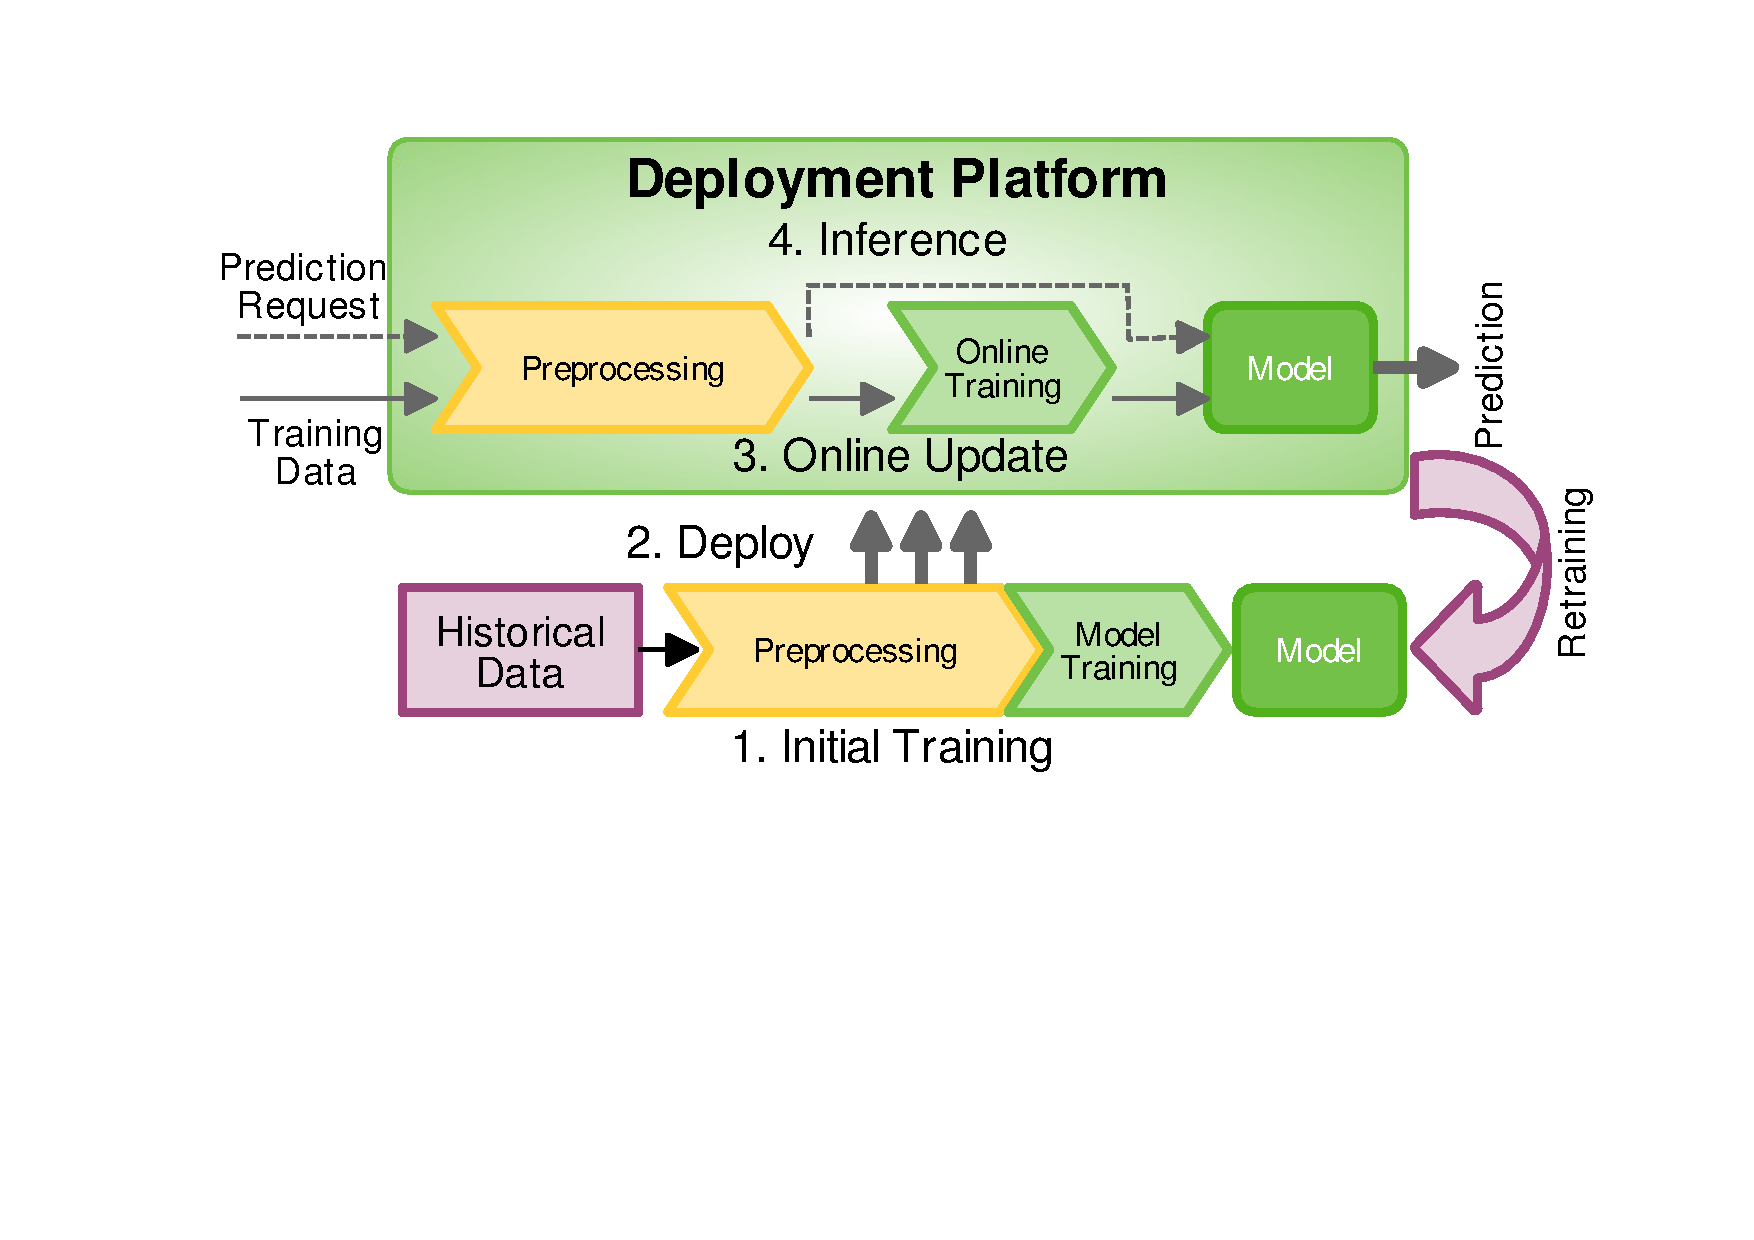
\includegraphics[width=\columnwidth]{../images/generic-motivational-example-v2.pdf}
%\caption{Periodical deployment of machine learning pipelines}
%\label{fig:motivational-example}
%\end{subfigure}%
%\begin{subfigure}{\columnwidth}
%\centering
%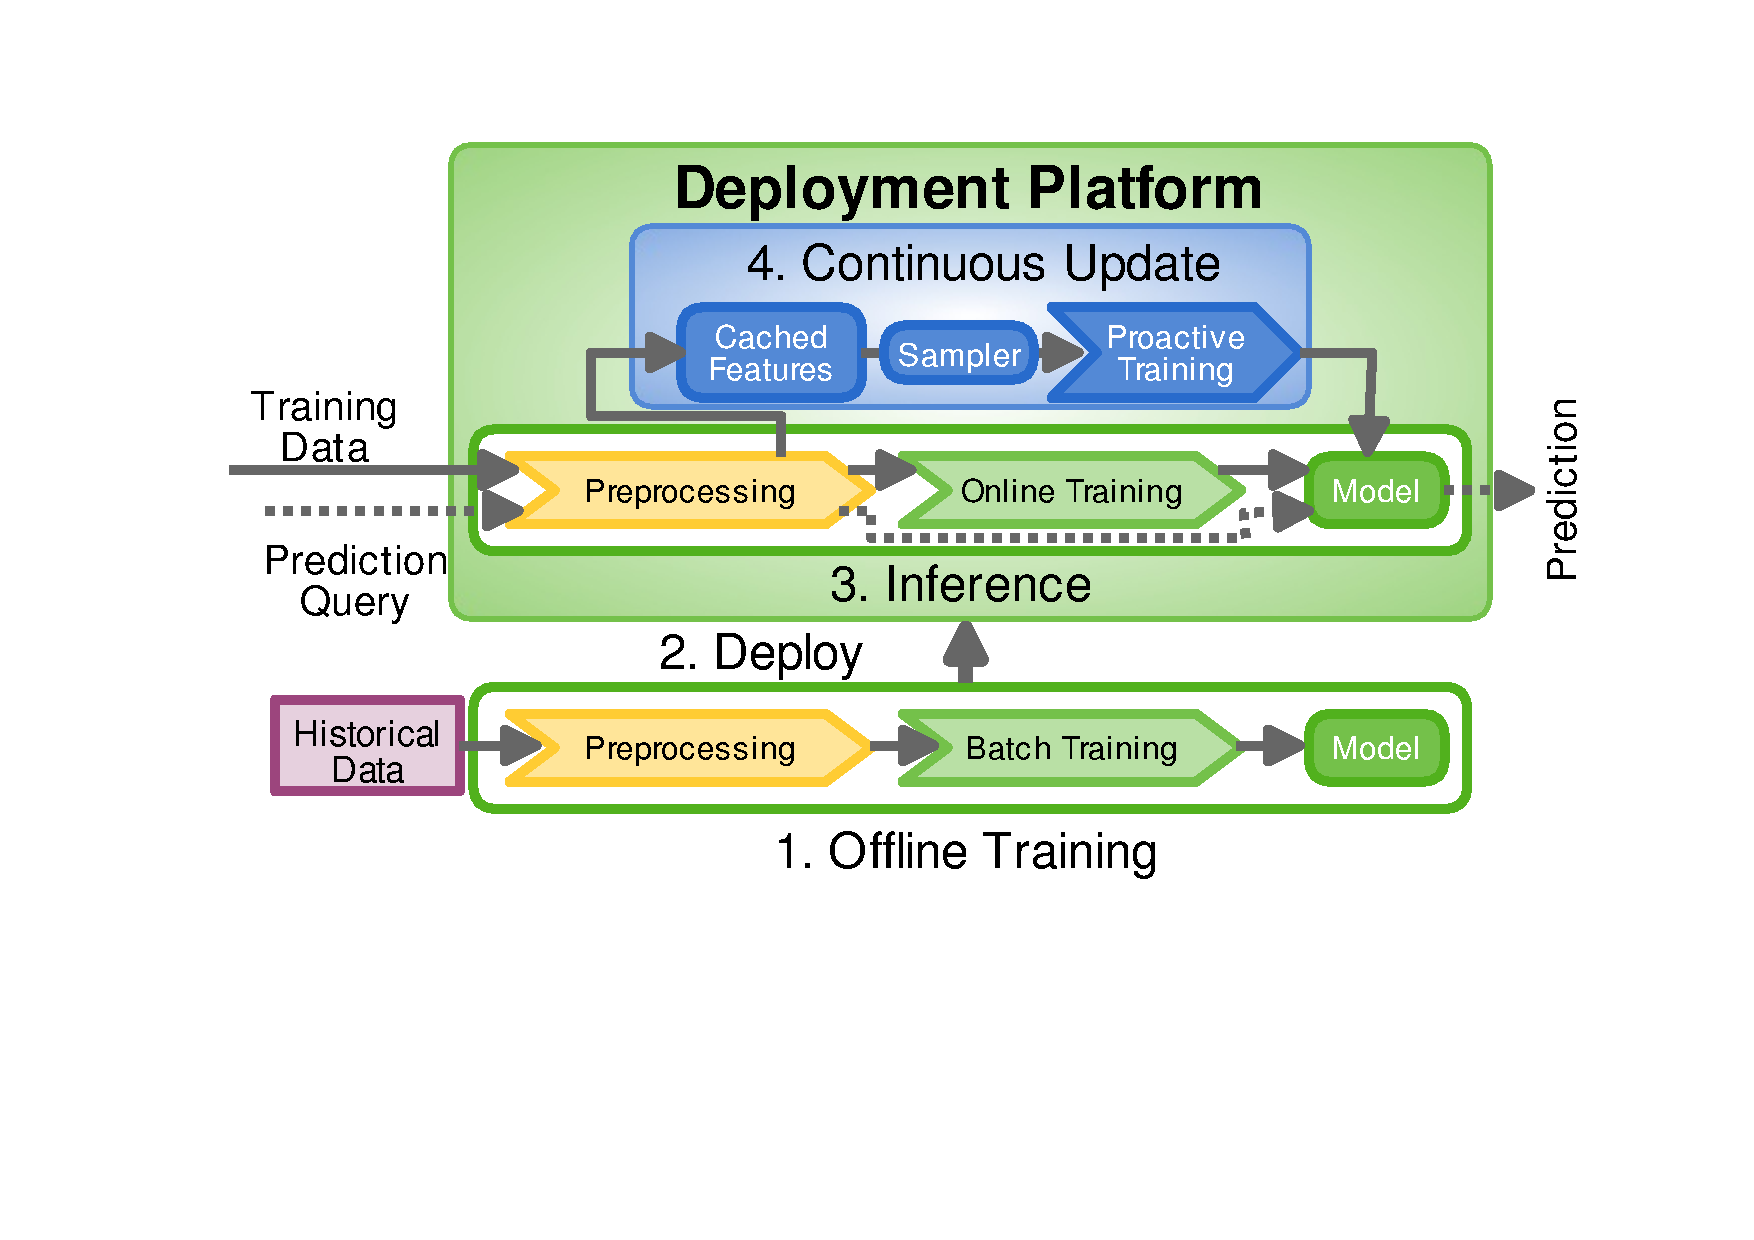
\includegraphics[width=\columnwidth]{../images/generic-improved-example-v2.pdf}
%\caption{Continuous deployment of machine learning applications}
%\label{fig:improved-example}
%\end{subfigure}
%\caption{Machine Learning Deployment Platforms}
%\label{deployment-processes}
%\end{figure*}
%Figure \ref{deployment-processes} shows the differences in deployment processes of the periodical and continuous training approaches.
%Figure \ref{fig:motivational-example} shows the process of the periodical deployment approach.
%The process starts with an offline training \circled{1}.
%During the offline training, a user designs a machine learning pipeline that consists of several data and feature preprocessing steps. 
%After the data preprocessing step, the user trains a machine learning model by utilizing a batch training algorithm.
%During the deployment step, the user deploys the model and the pipeline into the deployment platform \circled{2}.
%To perform inference, the deployment platform directs the incoming prediction queries through the preprocessing steps before utilizing the model to predict the label \circled{3}.
%During the online update step, the deployment platform directs the training data through the preprocessing steps of the pipeline and then, using an online training algorithm, the platform updates the model.
%Finally, the deployment platform accommodates periodical retraining of the pipeline by either automatically triggering a batch training or prompting the user to train and redeploy a new model to the deployment platform \circled{4}.
%During the periodical retraining, the deployment platform has to disable the online updating of the model.
%
%Figure \ref{fig:improved-example} shows how our continuous training approach improves the existing deployment process.
%Similar to the current deployment process, a user first trains a pipeline \circled{1} and deploy it into the deployment platform \circled{2}.
%The deployment platform utilizes the deployed pipeline and model to answer prediction queries and update the model using the incoming training data \circled{3}.
%After transforming the incoming data into a set of features, the deployment platform stores the transformed features inside a cache.
%During the proactive training, the platform samples the materialized features and computes the gradient using the sample.
%Finally, the platform updates the deployed model using the gradient \circled{4}.
%In the new deployment approach, the platform continuously updates the pipeline and the deployed model without requiring a full retraining over the historical data.
%As a result, the deployment platform ensures the model is always up-to-date.